\documentclass[dvipdfmx, titlepage, 11pt]{jsarticle}
\usepackage{tikz}
\usetikzlibrary{patterns}
\usetikzlibrary{intersections,calc,arrows}
\usepackage[top=20truemm,bottom=20truemm,left=15truemm,right=15truemm]{geometry}
\usepackage{enumerate}
\usepackage{multicol}
\usepackage{diagbox}
\usepackage{graphicx}

\makeatletter
\newcommand{\overarc}[1]{
  \setbox0\hbox{#1}%
  \ifdim\wd0<1em%
    \stackrel{\frown}{#1}%
  \else\ifdim\wd0<1.75em%
    \stackrel{\rotatebox{90}{\big)}}{#1}%
  \else\ifdim\wd0<2.5em%
    \stackrel{\rotatebox{90}{\Big)}}{#1}%
  \else\ifdim\wd0<3.25em%
    \stackrel{\rotatebox{90}{\bigg)}}{#1}%
  \else%
    \stackrel{%
      \rotatebox[origin=c]{90}{\mbox{%
        $\left.\vphantom{\rotatebox[origin=c]{90}{#1}}\right)$%
      }}%
    }{#1}%
  \fi\fi\fi\fi%
}
\makeatother

\newcommand{\ncircle}[1]{\textcircled{\scriptsize #1}}
\newcommand{\nbox}[1]{\fbox{\hspace{5pt} \textcircled{\scriptsize #1}\hspace{5pt} }}
\newcommand{\ebox}{\fbox{ \hspace{10pt} }}

\title{\Huge 数学}
\author{\LARGE 試験時間 : 50分}
\date{\LARGE 平成31年度筑波大附属高校\\[3cm] 大問は \fbox{\Large {\bf 1}} から \fbox{\Large {\bf 5}} まであります\\[0.5cm] 解答は解答用紙に記入して下さい}
\begin{document}
\maketitle

\newpage
\thispagestyle{empty}
 
\newpage

\newpage
\thispagestyle{empty}
 
\newpage

\setcounter{page}{1}
\noindent \fbox{\LARGE {\bf 1}}\hspace{10pt} 次の\textcircled{\scriptsize 1} 〜 \textcircled{\scriptsize 3}の \fbox{ \hspace{10pt} } にあてはまる数を求めなさい.
\begin{enumerate}[(1)]
\item 直線 $l : y = ax+b$がある. $l$と直線$y=1$に関して対称である直線を$m$とし, $m$と直線$x=1$に関して対称である直線を$n$とする.\\
  $m$が点$(-1,\ 4)$を通り, $n$が点$(5,\ -2)$を通るとき,\ $a =$ \fbox{\hspace{5pt} \ncircle{1} -- 1\hspace{5pt} } ,\ \ $b=$ \fbox{\hspace{5pt} \ncircle{1} -- 2\hspace{5pt} } である.\\[3.5cm]
  \begin{multicols}{2}
  \item 右の図のように, $\angle$A=$50^{\circ}$,\ \ $\angle$B=$60^{\circ}$,\ \ $\angle$C=$70^{\circ}$の$\triangle$ABCを, 頂点Cを中心として時計まわりに$25^{\circ}$回転させたとき,\ A,\ \ Bが移る点を, それぞれD,\ \ Eとする.\\
    ABとDEの交点をFとするとき, $\angle$BEC$+\angle$ECF$=$ \nbox{2} 度である.

    \begin{center}
      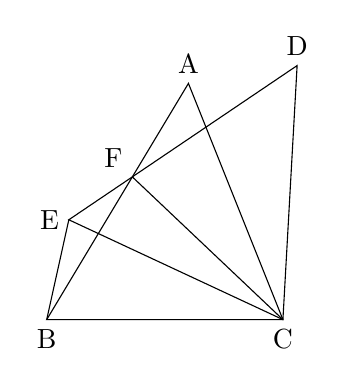
\begin{tikzpicture}
        \draw[name path=A] (0,0) node[below] {C}--(-1.2,3) node[above] {A}--(-3,0) node[below] {B}--cycle;
        \draw[rotate=-25, name path=B] (0,0)--(-1.2,3) node[above] {D}--(-3,0)node[left] {E}--cycle;
        \path[name intersections={of = A and B}];
        \draw (-3,0)--(155:3);
        \draw (0,0)--(intersection-3) node[above left] {F};
      \end{tikzpicture}
    \end{center}
  \end{multicols}
  \vspace{2cm}
  
\item 12321,\ \ 314413のように, 数字を逆から並べても元の数と同じになる数のことを回文数という.\\
  4桁の回文数のうち, 9の倍数であるものは \nbox{3} 個ある.
\end{enumerate}

\newpage

\begin{multicols}{2}
  \noindent \fbox{\LARGE {\bf 2}}\hspace{10pt} 右の図のように, 傾きが一定の緩やかな坂がある. この坂の上にボールを置いて静かに手をはなすとボールは坂を転がり落ちるが, 転がり始めてからの移動距離は, 転がる時間の2乗に比例する.\\[2cm]
  \begin{center}
    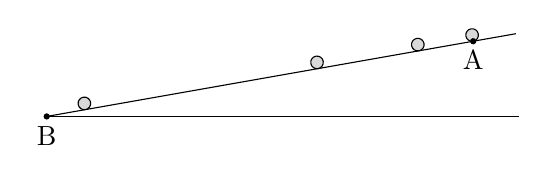
\begin{tikzpicture}
      \draw (0,0)--(6,0);
      \draw[rotate=10] (0,0)--(6.05,0);
      \draw[rotate=10, fill=gray!30] (0.5,0.08) circle[radius=0.08];
      \draw[rotate=10, fill=gray!30] (3.5,0.08) circle[radius=0.08];
      \draw[rotate=10, fill=gray!30] (4.8,0.08) circle[radius=0.08];
      \draw[rotate=10, fill=gray!30] (5.5,0.08) circle[radius=0.08];
      \fill (0,0) circle[radius=0.04];
      \fill[rotate=10] (5.5,0) circle[radius=0.04];
      \draw (10:5.5) node[below] {A};
      \draw (0,0) node[below] {B};
    \end{tikzpicture}
  \end{center}
\end{multicols}
Pさんはこの坂の上のA地点に立ち, そこにボールを置いて静かに手を離した. その2秒後, Pさんは一定の速さで坂を下りてボールを追いかけたところ, 追いかけ始めてから1秒後にボールを追い越したが, その後ボールに追い抜かれた. 追い抜かれた2秒後, 坂を下る速さを3倍にしたところ, 再びボールを追い越したが, 坂を下りきったB地点でちょうどボールに追いつかれた. このとき, 次の \ncircle{4} 〜 \ncircle{6} の \ebox にあてはまる数を求めなさい.
\begin{enumerate}[(1)]
\item Pさんが最初にボールに追い抜かれたのは, ボールが転がり始めてから \nbox{4} 秒後である.\\[3cm]
\item PさんがB地点においてボールに追いつかれたのは, ボールが転がり始めてから \nbox{5} 秒後である.\\[3cm]
\item 2地点A,\ B間の距離が40.5mであるとき, A地点を出発したときのPさんの速さは毎秒 \nbox{6} mである.
\end{enumerate}
\newpage

\begin{minipage}{0.7\hsize}
  \noindent \fbox{\LARGE {\bf 3}}\hspace{10pt} 右の絵のような正八面体のさいころがあり, それぞれの面に1から8までの数字が1つずつかかれている. このさいころを振ったときの「出た目」は, 上面にかかれている数で, 右の絵では8である. それぞれの目が出る確率は等しいものとする. 以下, このさいころを使用する.
\end{minipage}
\begin{minipage}{0.26\hsize}
  \begin{center}
    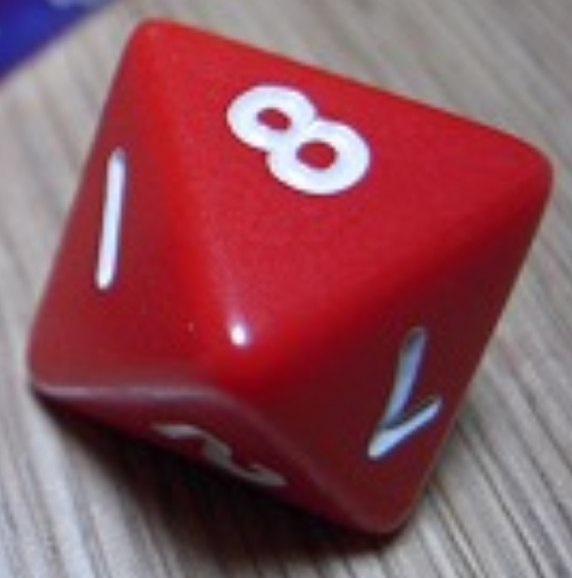
\includegraphics[width=2.6cm]{sai.png}
  \end{center}
\end{minipage}

\begin{minipage}{0.7\hsize}
  右の図のような正方形ABCDの周上を反時計まわりに動く点Pがある. 最初Pは頂点Aにあり, さいころを振って出た目と同じ数の辺の分だけ移動する. 例えば7の目が出た場合は, A$\to$ B $\to$ C $\to$ D $\to$ A $\to$ B $\to$ C $\to$ Dというように移動する. このとき, 次の \ncircle{7} 〜 \ncircle{9} の \ebox \ にあてはまる数を求めなさい.
\end{minipage}
\begin{minipage}{0.26\hsize}
  \begin{center}
    \begin{tikzpicture}[>=stealth, scale = 0.8]
      \draw (0,0) node[below] {B} -- (3,0) node[below] {C} -- (3,3) node[above] {D} -- (0,3) node[above] {A} -- cycle;
    \end{tikzpicture}
  \end{center}
\end{minipage}

\begin{enumerate}[(1)]
\item さいころを2回続けて振って移動した後, Pが頂点Aにある確率は, \nbox{7} である.
  \newpage
\item さいころのどれか1つの面に, 数字「0」のかかれたシールを貼る. もしこの面が出た場合, Pは移動しない.\\
  シールの貼ったさいころを2回続けて振って移動した後, Pが頂点Aにある確率が最も高くなるのは, シールを \nbox{8} の数字がかかれた面に貼ったときであり, そのときの確率は \nbox{9} である. ただし, シールを貼ってもそれぞれの目が出る確率は等しいものとする.
\end{enumerate}
\newpage

\begin{multicols}{2}
  \noindent \fbox{\LARGE {\bf 4}}\hspace{10pt} 点Oを中心とする球面上に4点A,\ B,\ C,\ Dがあり, $\triangle$ ABCと $\triangle$ BCDは1辺が6cmの正三角形, AD=$3\sqrt{6}$cmである. このとき, 次の\ncircle{10} 〜 \ncircle{12} の \ebox \ にあてはまる数を求めなさい.
  \begin{center}
    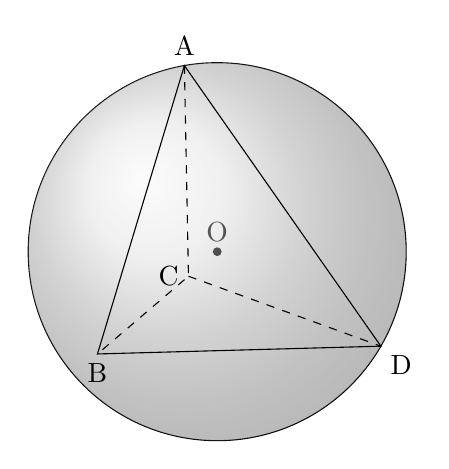
\begin{tikzpicture}[scale=0.8]
      \draw (0,0) circle[radius=3];
      \fill (0,0) node[above] {O} circle[radius=0.07];
      \shade[ball color=gray!40, opacity=0.4] (0,0) circle[radius=3];
      \draw (100:3) node[above] {A} -- (220.5:2.5) node[below] {B} -- (330:3) node[below right] {D}--cycle;
      \draw[dashed] (100:3)--(220.5:0.6) node[left] {C}--(220.5:2.5);
      \draw[dashed] (220.5:0.6) -- (330:3);
    \end{tikzpicture}
  \end{center}
\end{multicols}
\vspace{3cm}

\begin{enumerate}[(1)]
\item 四面体ABCDの体積は \nbox{10} cm${}^{3}$である.
  \newpage
\item 球Oの半径は \nbox{11} cmである.\\[7cm]
\item 3点O,\ \ C,\ \ Dを通る平面で四面体ABCDを切断して2つの立体に分けたとき, 小さい方の体積は \nbox{12} cm${}^{3}$である.
\end{enumerate}
\newpage
\begin{multicols}{2}
  \noindent \fbox{\LARGE {\bf 5}}\hspace{10pt} 右の図のように, 長さ6cmの辺ABを共有する正方形ABCDと正三角形AEBがある. 正方形の4頂点を通る円をO,\ \ 正三角形の3頂点を通る円をO$'$とし,\ \ 円Oの周上を動く点をP,\ \ 円O'の周上を動く点をQとする. ただし, 点P,\ \ Qは, 線分PQ(両端を除く)の上に点Bがあるように動くものとする. \\
  $\triangle$APQの面積を$S$(cm${}^{2}$)とするとき, 次の \ncircle{13} の \ebox \ \ にあてはまる数を求め, 解答欄 \ncircle{14}には指定された図形および文章を記入しなさい.
  \begin{center}
    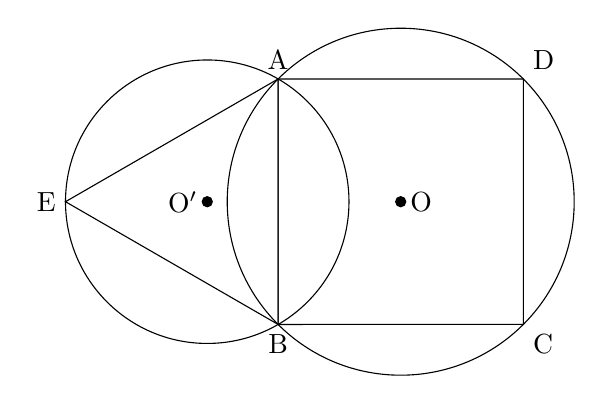
\begin{tikzpicture}[>=stealth, scale=1.8]
      \draw (0,0) circle[radius=1];

      \draw (60:1)node[above] {A}--(180:1) node[left] {E}--(300:1)node[below] {B}--cycle;
      \draw (1.365,0) circle[radius=1.224];
      \draw ($(45:1.224)+(1.365,0)$) node[above right] {D}--(60:1)--(300:1)--($(1.365,0)+(315:1.224)$)node[below right] {C}--cycle;

      \fill (0,0) node[left] {O$'$} circle[radius=0.04];
     \fill (1.365,0) node[right] {O} circle[radius=0.04];
    \end{tikzpicture}
  \end{center}
\end{multicols}
\begin{enumerate}[(1)]
\item 点Qが点Eと一致するとき, $S$ = \nbox{13} (cm${}^{2}$) である.\\[5cm]
\item $S$が最大となるときの$\triangle$APQを解答欄 \ncircle{14} の図(上の図と同じ図)にかき入れ, その三角形が最大である理由を関係に述べなさい. ただし, 証明は不要です.
\end{enumerate}
\newpage
\thispagestyle{empty}
 
\newpage
\newpage
\thispagestyle{empty}
 
\newpage

\end{document}
